This is the final iteration report for the course Problem Analysis and Software Design. Before we start the formal report, we'd like to address a couple of things.
First and foremost, the majority of the report was written by two students, Robbin de Groot (student A) and Nicu Ghidirimischi (student C). The remaining student B, Oliver Strik dropped the course the night before the iteration 2 deadline (around 11 PM, which caused us both quite some frustration). The lecturer(s) know about this now, and we have discussed the following plan of attack.
\begin{itemize}
	\item We continue to work on the report like we have always worked on it in pairs
	\item We leave out any trailing work of Oliver's
	\item Since we have interaction diagrams of his first use case, we slightly refine his use case in order to better update those interaction diagrams. This however is not a major refinement, as the interaction diagrams of B1 already got a sufficient grade (a 9 out of 10 to be precise).
	\item This entails that Oliver's work that is still in the report ought not to be graded, even though our interation diagrams depend on it.
\end{itemize}
We assume you still stand by these decisions and adhere to them during grading. Thank you.\\\\
\textsl{Workload Division Table}
\begin{center}\begin{tabular}{|l|l|l|l|}
\hline
 & Student A & Student B & Student C\\\hline
 Name: & Robbin de Groot & Oliver Strik & Nicu Ghidirimischi\\\hline
 Use case 1:& Add Item & Update Item & Delete Item\\\hline
 Use case 2:& Create Search Request & Update Search Request & Reserve Book\\\hline
 Use case 3:& Register Regular Customer & - & View administration  \\\hline
 Interaction Diagrams 1:& Update Item& - & Add Item\\\hline
 Interaction Diagrams 2:& Reserve Book & - & Delete Item\\\hline
 Interaction Diagrams 3:& View administration & - & Register Regular Customer \\\hline
 \end{tabular}\end{center}
 Note that, since Oliver Strik (student B) dropped out of the course, we did not follow the prescribed division of work. That is to say, both of the remaining students (Robbin (A) and Nicu (C)) each did 3 use cases and wrote 3 interaction diagrams. However, for example, the interaction diagram for C1 is also made by student C, which was not the intended way according to the table in nestor. We did this for completeness sake, since we could not rely on the work of Oliver being delived in time. We hope you accept this.\\\\
 \textsl{Message to Lecturers (next page)}
 \begin{figure}[H]
 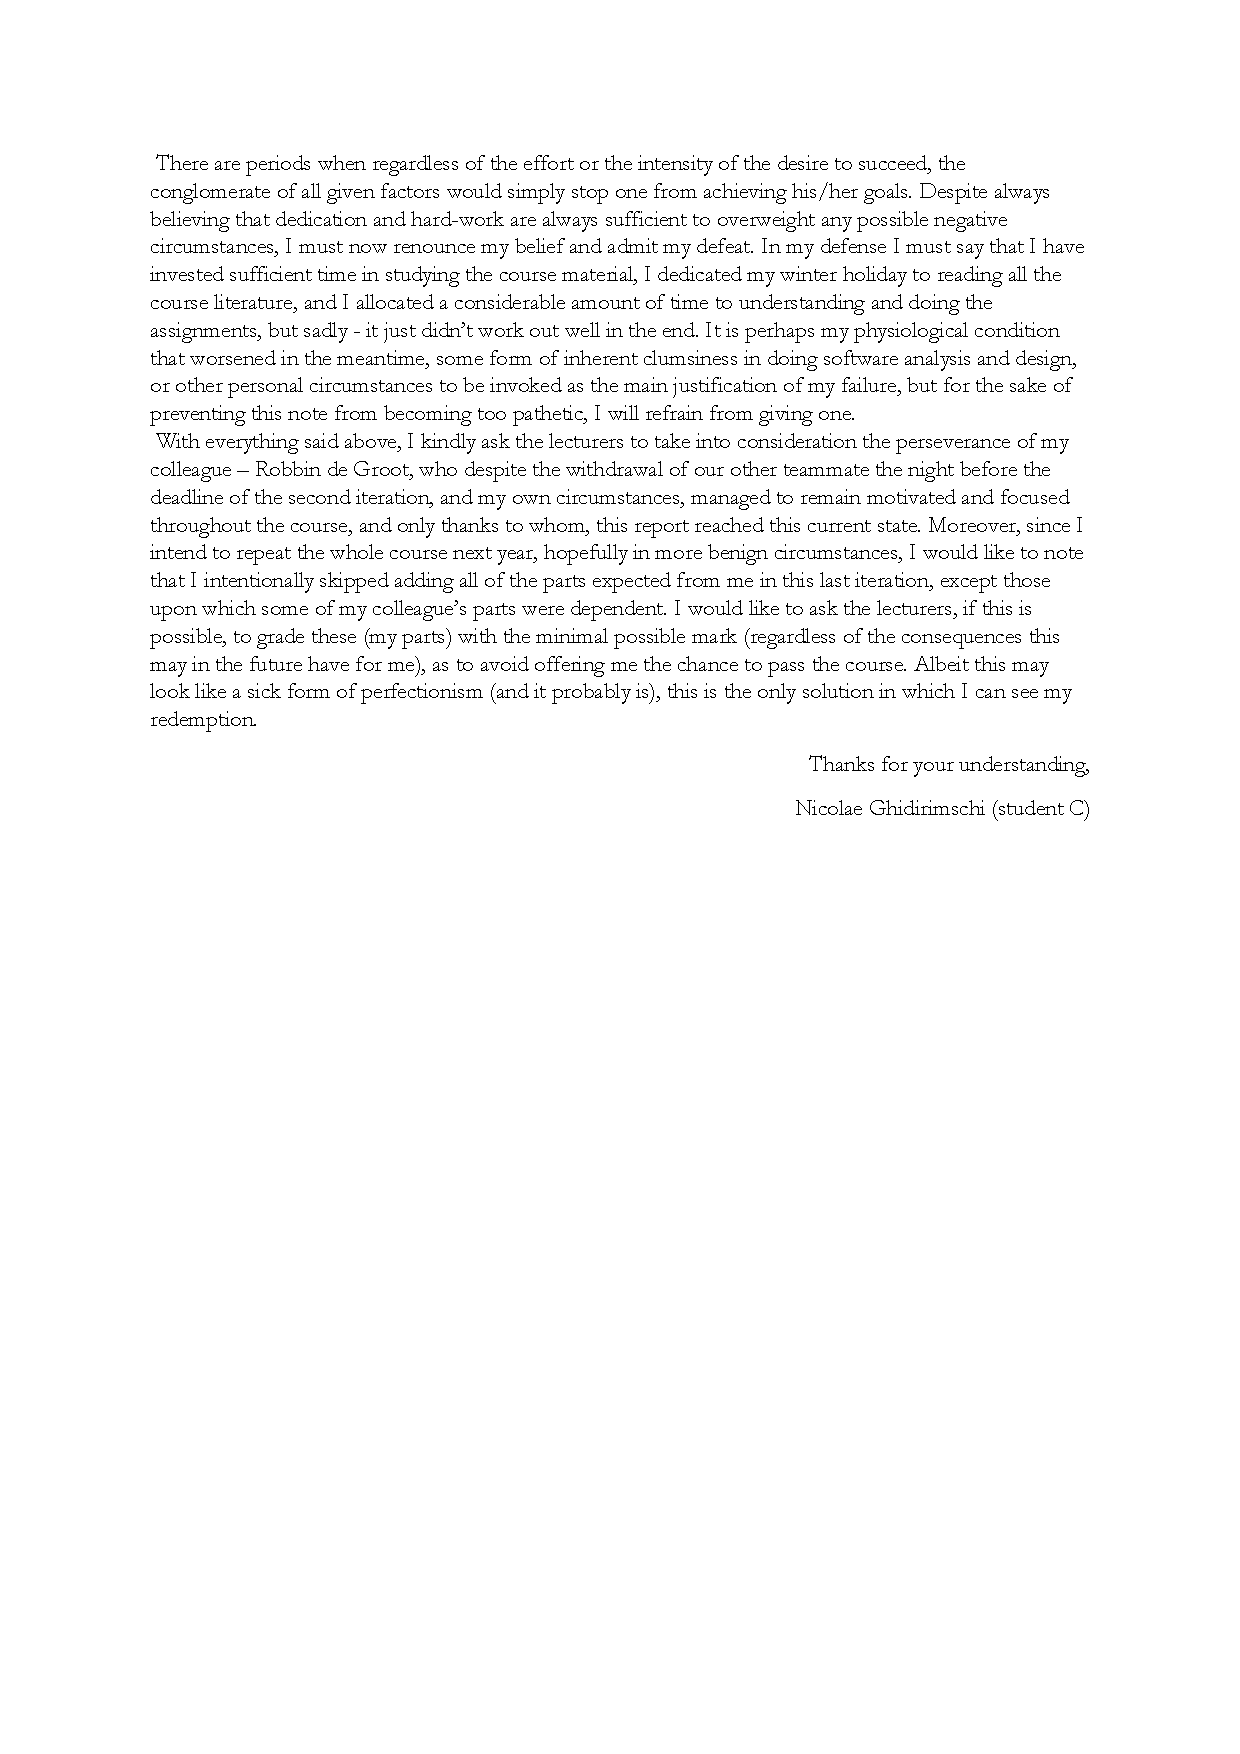
\includegraphics[scale = .8]{nicunote.pdf}
 \end{figure}
